\chapter{特殊相対性理論：基準系、同時性、ローレンツ変換}

相対性とは、物理法則がそれを記述するために用いる慣性系に依存しないという原理である。最初の課題は運動学である。すなわち、空間、時間、運動、同期の意味、および一つの慣性系から別の慣性系への変換である。力学はその後に来る。相対論的エネルギー、運動量、力、ニュートンの運動方程式の類似物、そして\(E=mc^2\)の意味である。その構造が確立すれば、一般相対性理論に概念的アプローチできる。曲がった時空、与えられた重力場中の粒子の運動、ブラックホール、宇宙の膨張を通じてであり、アインシュタインの場の方程式を解くという困難な問題から始めることなく。

概念的厳密さと数学的厳密さの区別は重要である。我々は故意に偽である近似を用いることはない。むしろ、重力場が時計、粒子、幾何学に何をするかに重点を置き、場の方程式の任意の解を構成するために必要な道具立ては後回しにする。特殊相対性理論はより明示的に扱わなければならない。その後の推論のすべてがその運動学に依拠しているからである。

したがって、出発すべき正しい場所は、有名な公式ではなく、観測者が場所と時間によって何を意味するかの正確な説明である。

\section{基準系とは物理的な座標系である}

空間が任意に細かい物差しの格子で満たされていると想像せよ。各格子点は三つの空間座標でラベル付けされ、各点には時計がある。棒と時計が一緒になって基準系を構成する。

\begin{definition}
\emph{事象}とは、一つの場所と一つの時間に起こるものである。一次元空間ではその座標は\((x,t)\)と書かれ、三次元では\((x,y,z,t)\)である。
\end{definition}

ニュートン物理学は強力な仮定を加える。すべての理想的な時計は一度で永久に同期できる。時間は普遍的である。時計は動かされてもよく、観測者は腕時計を持ち歩いてもよいが、誰もがどこでも同じ\(t\)に同意するとされる。これは絶対時間と呼ばれることがあり、神の時間、全世界のための一つの時計として思い描くことができる。

相対性原理はアインシュタインより古い。その自然な描像は、完全に滑らかなレールの上をあまりに一様に動くため何もガタガタ揺れない列車である。列車の中では、駅に停まっている列車でするのとまったく同じようにボールを投げて受け取ることができる。ジャグリングは驚くほど完全な小さな力学実験である。タイミング、重力、位置合わせ、軌道の繰り返し制御を必要とする。列車が一定速度で動くなら、それらの規則はどれも変わらない。真上に投げたボールは同じ手に戻る。列車がその下から滑り出ることはない。ガリレオはこの事実を認識し、ニュートンは運動法則において体系的に表現した。

ガリレオ以前には、動く列車はボールが空中にある間に進むはずであり、ジャグラーはそれを取り戻すために後ろや前へ手を伸ばさねばならないと推論する誘惑があった。誤りは、ボールが手を離れるときすでに列車の水平速度を共有していることを忘れることである。滑らかに動く車両内に限定された実験は、絶対的静止の特別な状態を明らかにしない。観測できるのは二つの列車の間の相対運動だけである。

したがって、静止した列車と一様に動く列車は二つの慣性系である。アインシュタイン以前には、それらはガリレイ変換によって関係づけられていた。

\section{時空を描く}

ここでは\(y\)と\(z\)を一時的に抑制し、時間を縦に、位置\(x\)を横に描く。図中の各点は事象である。線\(x=0\)は空間原点の履歴、すなわち\emph{世界線}である。隣接する縦線\(x=1,2,3,\ldots\)は他の格子点の世界線である。横線は共通の時間をもつ事象の集合である。

\begin{figure}[H]
\centering
\includegraphics[width=0.62\textwidth]{lecture_01_figure_02.png}
\caption{静止系の時間軸と空間格子の最初の世界線。}
\lectureframe{00:16:38}
\end{figure}

同じ構成は理想化された図ではより明確である：

\begin{figure}[H]
\centering
\begin{tikzpicture}[scale=0.95]
\draw[->] (-1.2,0) -- (5.2,0) node[right] {$x$};
\draw[->] (0,-0.2) -- (0,4.8) node[above] {$t$};
\foreach \x in {-1,1,2,3,4}
  \draw[gray!65] (\x,0) -- (\x,4.4);
\foreach \y in {1,2,3,4}
  \draw[gray!65] (-1.0,\y) -- (4.4,\y);
\fill (0,0) circle (1.5pt);
\node[below left] at (0,0) {$0$};
\node[left] at (0,1) {$1$};
\node[left] at (0,2) {$2$};
\node[left] at (0,3) {$3$};
\node[below] at (1,0) {$1$};
\node[below] at (2,0) {$2$};
\node[below] at (3,0) {$3$};
\end{tikzpicture}
\caption{静止した時空格子。縦線は一定の位置を、横線は一定の時間をもつ。}
\end{figure}

格子は想像上のものであり、その間隔は任意である。メートル、センチメートル、ミクロン、あるいは物理的に意味をなすさらに小さな間隔のいずれでもよい。その目的は、すべての事象に正確な座標を割り当てることである。

「基準系」という語は今や操作的な内容を持つ。それは単なる視点や、ある方向を見ている人ではない。それは拡張された座標装置である。事象が与えられれば、局所的な物差しがそれがどこで起こったかを指定し、局所的な時計がいつ起こったかを指定する。そうすれば他の物理量を系の間で比較できる。粒子の位置と速度、そのエネルギー、おそらく物体の温度、そして最終的にはその運動量と力である。最も単純な比較は\(x\)と\(t\)を含むものであるから、そこから始める。

次に、正の\(x\)方向に一定の速度\(v\)で運動する列車の上に第二の格子を置く。原点は\(t=0\)で一致するように選ぶ。運動する原点はそのとき次に従う。
\begin{equation}
x=vt.
\end{equation}
列車に固定された他のすべての点は、平行に傾いた世界線に従う。この傾きは、時間が経過するにつれて列車が位置を変えるという幾何学的な陳述にすぎない。

列車の後端の点がプライム付き原点であるとする。\(t=0\)においてそれは駅の原点と一致する。より後の時刻\(t\)において、その静止座標は\(vt\)である。したがって座標\(x\)にある近くの事象は、列車の原点からわずか\(x-vt\)しか離れていない。これが、この変換が恣意的な代数規則ではなく引き算である理由である。

\((x,t)\)を駅系における事象の座標、\((x',t')\)を列車系におけるその座標とする。ガリレオとニュートンは普遍時間を保持する。
\begin{equation}
t'=t.
\end{equation}
時間\(t\)の間に、運動する原点は\(vt\)だけ進むので、その原点から事象までの距離は
\begin{equation}
x'=x-vt.
\end{equation}
である。合わせると、
\begin{align}
t'&=t, & x'&=x-vt.
\label{eq:galilean-forward}
\end{align}
プライムなしの座標について解くと逆変換が得られる。
\begin{align}
t&=t', & x&=x'+vt'.
\label{eq:galilean-inverse}
\end{align}

\begin{figure}[H]
\centering
\includegraphics[width=0.72\textwidth]{lecture_01_figure_03.png}
\caption{二つの時空格子の隣に書かれたガリレイ変換。}
\lectureframe{00:21:57}
\end{figure}

最初の組は、運動する観測者に、静止した観測者から与えられた座標をどのように変換するかを教える。逆の組は逆に変換し戻す。記述間のこの相互的な変換が、ガリレイ相対性の数学的内容である。

逆の空間の式における置き換え\(t\to t'\)が無害であるのは、ガリレイ理論がすでに\(t=t'\)を宣言しているからにすぎない。この仮定に今気づいておくことは有用である。アインシュタインの理論では二つの時間座標が異なるものになり、そのような置き換えはもはや自動的にはできない。

\begin{classroomqa}
\audiencequestion{時計を持ち去ってから再び持ち帰ったとき、その運動が最初に時計を速め、次に遅くして、時計を比較するときに効果を隠したのではないと、どうして知ることができるだろうか。
\lecturetimestamp{00:23:09}}
\lecturerresponse{ガリレオは現代的な精度で普遍時間を確立できなかったであろう。それは物理的な推測であった。我々はその推測を多くの方法で検証できる。良い時計を反対方向に持ち運び、北--南の旅だけでなく東--西の旅も繰り返し、一方の時計を他方の周りで動かし、あるいは時計を一緒にすることなく時刻信号を交換する。通常の速度では、そのようなすべての検証は非常に高い精度で一致する。十分に正確な時計または十分に大きな速度では、小さな不一致が現れる。普遍時間のこの失敗は実験の欠陥ではなく、特殊相対性理論が説明しなければならない現象の一つである。}
\end{classroomqa}

\section{ガリレイ不変量とニュートンの法則}

不変量とは、議論しているすべての慣性観測者が一致する量である。座標それ自体は不変である必要はない。重要なのは、それらから組み立てられた法則が同じ形を保つかどうかである。

この語は名詞としても形容詞としても用いられる。数が不変量であり得るし、方程式が変換の下で不変であり得る。不変な量と不変な法則の区別は、よくある混乱を防ぐ。相対性理論は、すべての観測者がすべてについて同じ座標を得ると主張しているのではない。それは、彼らの測定を結びつける物理法則が同じ形を持つと主張しているのである。

位置\(x_1\)と\(x_2\)にある二つの同時事象を取る。式~\eqref{eq:galilean-forward}は次を与える。
\begin{align}
x_1'&=x_1-vt,\\
x_2'&=x_2-vt.
\end{align}
したがってそれらの隔たりは
\begin{equation}
x_2'-x_1'=(x_2-vt)-(x_1-vt)=x_2-x_1.
\end{equation}
である。ガリレイ物理学では、個々の位置は不変でなくても、同じ時刻に起こる事象間の距離は不変である。

\begin{classroomqa}
\audiencequestion{その引き算における\(t\)の二つの出現は本当に同じ時刻だろうか。
\lecturetimestamp{00:28:16}}
\lecturerresponse{はい。我々は二つの事象を意図的に\((x_1,t)\)と\((x_2,t)\)に選んだ。それらは一つの水平な等時刻線上にある。したがって共通項\(vt\)は相殺される。もし事象が異なる時刻に起こったなら、この議論は不変な空間的隔たりを確立しないであろう。}
\end{classroomqa}

次に、粒子を軌道\(x(t)\)によって記述する。列車の観測者は
\begin{equation}
x'(t)=x(t)-vt.
\end{equation}
を割り当てる。1回微分すると、おなじみの速度の加法則
\begin{equation}
\frac{dx'}{dt}=\frac{dx}{dt}-v.
\end{equation}
が得られる。位置と速度は座標系に依存する。矢のそばを移動する観測者は、線路のそばに立つ観測者よりも矢がゆっくり進むのを見る。

もう一度微分する。相対速度\(v\)は一定であるから、
\begin{equation}
\frac{d^2x'}{dt^2}=\frac{d^2x}{dt^2}.
\end{equation}
加速度はガリレイ変換の下で不変である。このことは、ニュートンの法則がなぜ位置や速度ではなく加速度を用いて書かれるのかを強く示唆している。

これは観測される物体の加速度であり、列車の観測者の加速度ではない。両方の座標系は慣性系であるから、どちらの座標系も他方に対して加速していない。物体はどちらの記述の中でも左または右に加速しうるし、2人の観測者は、物体の位置と速度については一致しないにもかかわらず、その加速度の値については一致する。

2つの粒子が互いに力を及ぼし合い、その力が同時的な隔たりのみに依存するとしよう。その隔たりは不変であるから、力も不変である。質量もまた本質的で座標系に依存しない性質であるならば、すべての慣性観測者は
\begin{equation}
F=ma
\end{equation}
をまったく同じ形で書くことができる。ニュートン力学はガリレイ変換の下で不変である。それは単にもっともらしいだけでなく、通常の速度の領域の全体にわたって極めて正確である。

この議論は、大きさが距離の関数であるような、ニュートン重力や静電場のようなおなじみの中心力に当てはまる。すべてのガリレイ観測者は共通の時刻におけるその距離について一致するので、力についても一致する。力と加速度が固定されれば、整合性は彼らが質量についても一致することを要求する。1キログラムの物体は、列車で運ばれても1キログラムの物体のままである。\(F=ma\)の中のすべての記号が同じ不変な構造に当てはまる。

\section{光はガリレイの規則に当てはまらない}

電磁気学が困難を生み出す。マクスウェル方程式は、空虚な空間を確定した速さ\(c\)で伝わる波を予言する。マクスウェル方程式が自然の法則であり、自然の法則がすべての慣性系で同じであるならば、すべての慣性観測者は同じ\(c\)を得なければならない。

ガリレイの運動学は別のことを予言する。静止系で右向きに進む光パルスは次を満たす。
\begin{equation}
x=ct.
\end{equation}
空間の変換を適用すると次が得られる。
\begin{equation}
x'=x-vt=(c-v)t.
\end{equation}
\(t'=t\)であるから、列車の観測者は速さ\(c-v\)を測定することになる。

矛盾は鋭く述べることができる。マクスウェル方程式がその形を保つならば、それらはプライム系で\(c\)を予言する。ガリレイ変換が保たれるならば、それは\(c-v\)を予言する。\(v\ne0\)であるとき、両方が厳密でありうることはない。

この結果は、光が媒質中の通常の波のように振る舞うならば、まったく自然に見える。水面波とともに動く船は、より低い相対波速度を測る。静止した空気中を動く聴者は、空気に対する聴者の運動だけずれた音速を測る。したがって19世紀の物理学者たちは、優先的な静止状態、すなわちマクスウェル方程式が最も単純な形をとり、光が\(c\)で進むエーテル系へと導かれた。そのような優先的な系に対する運動を検出するために設計された実験は、対応する効果を何も見いださなかった。

可能な実験配置はいくつかあったが、それらの共通の目的は、異なる運動状態または運動方向にある観測者について光の伝播を比較することであった。いずれも予想されたガリレイ的ずれを明らかにしなかった。この失敗は小さな技術的厄介事ではなかった。それは、相対性原理、マクスウェル方程式、そして受け継がれた空間と時間の概念の間の選択を迫った。

アインシュタインはこの対立にいっそう直接的に取り組んだ。若いころ彼は光波を追いかけることを想像した。もしそれに追いつくことができれば、その振動する電磁的パターンは空間に凍りついて静止するであろうが、マクスウェル方程式はそのような静止した光波を許さない。彼はマクスウェルの理論と相対性原理を基本的なものとして扱い、次にわれわれの座標に隠された仮定を再検討することを選んだ。

この再構成は2つの要請に基づいている。
\begin{enumerate}
\item 物理法則はすべての慣性系で同じ形をとる。
\item 真空中の光はすべての慣性系で同じ速さ\(c\)をもつ。
\end{enumerate}

第2の要請はガリレイ変換と共存できない。速度の加法則よりも深い何かが変わらなければならない。アインシュタインの経済的な選択は、2つの要請を保ち、一見無害なガリレイの式\(t'=t\)を再検討することである。

\section{遠方の時計の同期}

空間的な距離は棒で配置できるが、離れた時計には同期の規約が必要である。中点にいる観測者から等距離に二つの時計を置く。各端点の時計が定められた時刻を指したとき、その時計に閃光を発させるとする。二つの閃光が同時に中点へ届けば、端点の時計は同期していると呼ぶ。一方の閃光が先に届けば、対応する時計を調整し、手順を繰り返す。

\emph{中点}という語は、その座標系ですでに配置された棒を用いて定義される。したがってこの判定には二つの別個の要素が含まれる。端点からの空間的距離が等しいことと、信号の到着時刻が等しいことである。どちらの要素も落としてよいものではない。この手順を格子全体で繰り返すことで、ニュートンが単に仮定していた水平な等時線が与えられる。

この定義が光を用いるのは、公準がすべての慣性系で光に同じ速さを割り当てているからである。すべての隣接する対についてこのように扱えば、格子全体が同期した時計の族を備えることになる。

次に、第二の格子を第一の格子に対して運動させる。運動する装置の中点は、それ自身の座標系では二つの運動する端点の中間に留まる。しかし静止した装置に対しては、一方の到来する閃光へ向かい、他方から遠ざかる。静止した時計に従って同時に発せられた閃光は、運動する中点に同時には届かない。運動する観測者は同じ中点と光の規則を適用するので、その観測者はそれらの発光を同時とは呼べない。各座標系は自身の時計を首尾一貫して同期させるが、二つの同期は一致しない。

これは光の有限な伝播時間によって生じる目の錯覚ではない。各観測者は光が届くのに時間がかかることを知っており、同じ速さ\(c\)を用いてそれを補正する。それでも不一致は残る。なぜなら観測者たちは同じ遠方の事象の対を同時なものとして選ばないからである。同時性の見かけだけでなく、同時性そのものが相対的である。

\begin{classroomqa}
\audiencequestion{光ではなく音で時計を同期させれば、この結論を避けられるだろうか。
\lecturetimestamp{00:49:03}}
\lecturerresponse{音は空気が静止している座標系では同期信号として機能するが、その測定される速さはすべての慣性系で同じではない。静止した空気の中を進む開放的な列車は、音を伝える媒質に対して運動しているので、そこでは前方と後方の音信号は対称には振る舞わない。光は公準によって異なる。すなわち、その静止系が一人の観測者を選び出すような検出可能な光の媒質は存在しない。したがって我々は光を用い、その帰結を追う。}
\end{classroomqa}

定性的な不一致は明らかである。次に、運動する観測者がどの事象を同時と呼ぶかを正確に計算する。

\section{光線による作図}

作図には、次の単位を選ぶと便利である。
\begin{equation}
c=1.
\end{equation}
このとき距離の一単位は、光が時間の一単位で進む距離である。すなわち光秒と秒、あるいは光年と年を組にする。空間と時間は同じ単位を持ち、速度は無次元となり、光線は\(45^\circ\)に現れる。右向きの光線は
\begin{equation}
x=t+d,
\end{equation}
であり、左向きの光線は
\begin{equation}
x=-t+d'.
\end{equation}
である。原点を通る二つの光線は単に\(x=t\)と\(x=-t\)である。光より遅い物体に属する時間的軌道は、垂直軸に近い側にある。仮想的な超光速の軌道は、水平軸に近い側にある。

図中の角度は、この単位の選択によって初めて意味を持つ。メートルと秒では、光線は一秒間にほぼ\(3\times10^8\)メートルを進むので、ほとんど水平に見えるであろう。距離に光秒を選ぶと水平軸が再スケールされ、因果的な幾何学が見えるようになる。

運動する格子の中の三本の平行な世界線を考える。
\begin{equation}
x=vt,\qquad x=vt+L,\qquad x=vt+2L.
\label{eq:moving-worldlines}
\end{equation}
中央の世界線は、二つの外側の点の間で同時性を判定する観測者に属する。三つの点はすべて一様に運動し、プライム付きの座標系でそれらの相対的な配置を保つ。

\begin{figure}[H]
\centering
\includegraphics[width=0.72\textwidth]{lecture_01_figure_04.png}
\caption{前方の光線\(x=t\)が中央の運動する世界線と出会う。}
\lectureframe{01:02:33}
\end{figure}

完全な幾何学は、黒板の前に立つ人の妨げなしに描くことができる。

\begin{figure}[H]
\centering
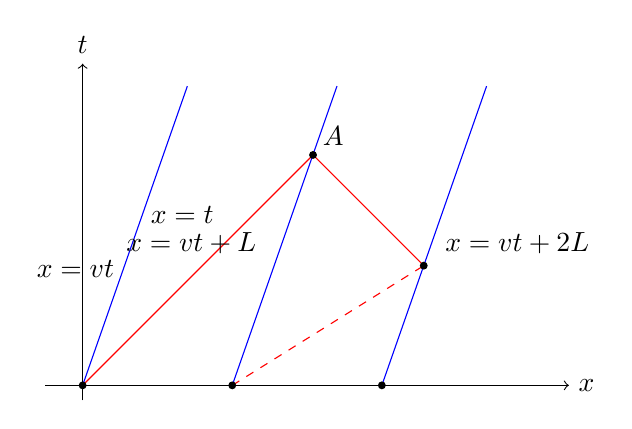
\begin{tikzpicture}[scale=0.95]
\draw[->] (-0.5,0) -- (6.5,0) node[right] {$x$};
\draw[->] (0,-0.2) -- (0,4.3) node[above] {$t$};
\draw[blue] (0,0) -- (1.4,4.0);
\draw[blue] (2.0,0) -- (3.4,4.0);
\draw[blue] (4.0,0) -- (5.4,4.0);
\draw[red] (0,0) -- (3.08,3.08);
\draw[red] (3.08,3.08) -- (4.56,1.60);
\draw[red,dashed] (2.0,0) -- (4.56,1.60);
\fill (0,0) circle (1.5pt);
\fill (2.0,0) circle (1.5pt);
\fill (4.0,0) circle (1.5pt);
\fill (3.08,3.08) circle (1.5pt);
\fill (4.56,1.60) circle (1.5pt);
\node[left] at (0.55,1.55) {$x=vt$};
\node[left] at (2.45,1.9) {$x=vt+L$};
\node[right] at (4.72,1.9) {$x=vt+2L$};
\node[left] at (1.88,2.28) {$x=t$};
\node[above right] at (3.08,3.08) {$A$};
\end{tikzpicture}
\caption{光信号が運動する座標系の同時線を決定する。}
\end{figure}

原点から右向きの光線を送る。\(A\)を、それが中央の世界線と交わる点とする。\(A\)における二つの方程式は
\begin{align}
x&=t,\\
x&=vt+L.
\end{align}
である。代入すると
\begin{equation}
t=vt+L,
\end{equation}
となり、したがって
\begin{equation}
t_A=x_A=\frac{L}{1-v}.
\label{eq:point-a}
\end{equation}

\(A\)から、左向きに進む光線を右端の運動する世界線までさかのぼる。その方程式は次の形をとる。
\begin{equation}
x+t=b.
\end{equation}
\(A\)を通るので、式~\eqref{eq:point-a}が定数を定める。
\begin{equation}
b=x_A+t_A=\frac{2L}{1-v}.
\end{equation}
したがって後ろ向きの光線は次を満たす。
\begin{equation}
x+t=\frac{2L}{1-v}.
\label{eq:backward-ray}
\end{equation}

右端の世界線との交点は次から従う。
\begin{align}
x+t&=\frac{2L}{1-v},\\
x&=vt+2L.
\end{align}
\(x\)を消去すると、
\begin{align}
(1+v)t
  &=2L\left(\frac{1}{1-v}-1\right)\\
  &=\frac{2Lv}{1-v},
\end{align}
よって
\begin{equation}
t=\frac{2Lv}{1-v^2}.
\end{equation}
\(x=vt+2L\)に代入すると次が得られる。
\begin{equation}
x=\frac{2L}{1-v^2}.
\end{equation}
座標そのものよりもそれらの比の方が重要である。
\begin{equation}
\frac{t}{x}=v.
\end{equation}
したがって、運動する時計によれば原点と同時であるすべての事象は次上にあり、
\begin{equation}
t=vx,
\label{eq:simultaneity-c-one}
\end{equation}
一方、運動する原点は次に従う。
\begin{equation}
x=vt.
\label{eq:moving-time-axis}
\end{equation}
二つの軸は\(45^\circ\)の光線のまわりに対称的に傾いている。

\(x=vt\)上のすべての点は同じプライム付き位置\(x'=0\)をもち、一方それらのプライム付き時間は変化する。\(t=vx\)上のすべての点は同じプライム付き時間\(t'=0\)をもち、一方それらのプライム付き位置は変化する。したがって一方の線はプライム付き時間軸であり、他方はプライム付き空間軸である。長い信号の構成は二番目の線を決定するために必要であった。それは運動する世界線だけから推論することはできなかった。

式~\eqref{eq:simultaneity-c-one}で通常の単位を復元するには次が必要である。
\begin{equation}
t=\frac{v}{c^2}x.
\label{eq:simultaneity-dimensional}
\end{equation}
因子\(c^2\)は、ニュートン的な描像が日常生活で非常によく成り立つ理由を説明する。\(c\)に比べて極めて小さい速度では、運動する同時線の傾きはきわめて小さい。

\begin{figure}[H]
\centering
\includegraphics[width=0.72\textwidth]{lecture_01_figure_05.png}
\caption{\(c=1\)のもとで、プライム付き時間軸と同時軸は光線に関して対称である。}
\lectureframe{01:15:40}
\end{figure}

\begin{figure}[H]
\centering
\begin{tikzpicture}[scale=1.0]
\draw[->] (-2.2,0) -- (5.2,0) node[right] {$x$};
\draw[->] (0,-0.2) -- (0,4.9) node[above] {$t$};
\draw[red] (0,0) -- (3.9,3.9);
\draw[red] (0,0) -- (-1.8,1.8);
\draw[blue] (0,0) -- (1.8,4.5);
\draw[blue,dashed] (0,0) -- (4.5,1.8);
\node[right] at (3.9,3.9) {$x=t$};
\node[left] at (-1.8,1.8) {$x=-t$};
\node[above] at (1.8,4.5) {$x'=0$};
\node[right] at (4.5,1.8) {$t'=0$};
\end{tikzpicture}
\caption{\(c=1\)単位でのプライム付き軸と不変な光線。}
\end{figure}

\section{ローレンツ変換の導出}

幾何学は各プライム付き座標がどこで消えるかを定める。運動する時間軸\(x=vt\)に沿って、\(x'=0\)でなければならない。運動する同時軸\(t=vx\)に沿って、\(t'=0\)でなければならない。それらの零点集合をもつ最も一般的な線形関係は次のように書ける。
\begin{align}
x'&=\frac{x-vt}{F(v)},\\
t'&=\frac{t-vx}{G(v)}.
\label{eq:fg-ansatz}
\end{align}
因子\(F\)と\(G\)は、軸がすでに位置づけられていても、プライム付き座標の目盛りがガリレイ的な目盛りと異なることを許す。線形性は空間と時間の一様性から従う。実験を平行移動しても変換則は変わらないからである。\editorialnote{この短い線形性の議論は、黒板での導出で暗黙に用いられていた仮定を明示する。}

この段階で、幾何学は多くを教えてくれたが、すべてではない。分子は軸の傾きを定める。それらはそれらの軸に沿った単位間隔を定めない。その残りの目盛り情報こそが、まさに\(F(v)\)と\(G(v)\)が表すものである。

ここで光速度の不変性を課す。\(x=t\)に従う右向きの光線はまた\(x'=t'\)にも従わなければならない。その光線に沿って、
\begin{align}
x'&=\frac{(1-v)t}{F(v)},\\
t'&=\frac{(1-v)t}{G(v)}.
\end{align}
光線上のすべての点に対する等号は次を要求する。
\begin{equation}
F(v)=G(v).
\end{equation}
したがって次のように書いてよい。
\begin{align}
x'&=\frac{x-vt}{F(v)},\\
t'&=\frac{t-vx}{F(v)}.
\label{eq:common-f}
\end{align}

この段階は、この代数において最初の真にアインシュタイン的な要請を用いる。同じ幾何学的な線が両方の観測者にとって光線であるので、\(c=1\)のとき、二つのプライム付き座標はそれに沿って等しく増加しなければならない。二つの方程式で因子が異なれば、プライム付き速度は1と異なることになる。

未知の関数が一つ残る。式~\eqref{eq:common-f}に\(F(v)\)を掛けると、
\begin{align}
F(v)x'&=x-vt,\\
F(v)t'&=t-vx.
\end{align}
第二の方程式に\(v\)を掛けて第一の方程式に加えると\(t\)が消去され、次が得られる。
\begin{equation}
(1-v^2)x=F(v)(x'+vt').
\end{equation}
同様に、
\begin{equation}
(1-v^2)t=F(v)(t'+vx').
\end{equation}
したがって逆変換は次である。
\begin{align}
x&=\frac{F(v)}{1-v^2}(x'+vt'),\\
t&=\frac{F(v)}{1-v^2}(t'+vx').
\end{align}

相対性原理は二つの系を相互的にする。駅が列車の動きを\(+v\)で見るなら、列車は駅の動きを\(-v\)で見る。したがって逆方程式は、\(v\)の符号を反転させた、順方向の方程式と同じ形をもたなければならない。それらの前因子は次を満たさなければならない。
\begin{equation}
\frac{F(v)}{1-v^2}=\frac{1}{F(v)}.
\end{equation}
ゆえに
\begin{equation}
F(v)^2=1-v^2,
\end{equation}
であり、\(v=0\)における恒等変換との連続性が正の根を選ぶ。
\begin{equation}
F(v)=\sqrt{1-v^2}.
\end{equation}

特定の光パルスに何も合わせていない。結果は、同期によって定まる軸、光の共通速度、およびどちらの慣性系も他方より特権的でないという要請から従う。

\(c=1\)とする単位でのローレンツ変換は次である。
\begin{align}
x'&=\frac{x-vt}{\sqrt{1-v^2}},\\
t'&=\frac{t-vx}{\sqrt{1-v^2}}.
\label{eq:lorentz-c-one}
\end{align}
その逆変換は次である。
\begin{align}
x&=\frac{x'+vt'}{\sqrt{1-v^2}},\\
t&=\frac{t'+vx'}{\sqrt{1-v^2}}.
\end{align}

\begin{figure}[H]
\centering
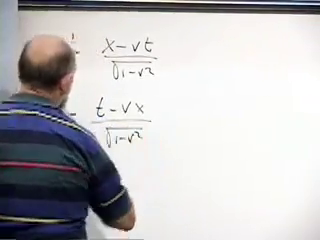
\includegraphics[width=0.76\textwidth]{lecture_01_figure_06.png}
\caption{黒板上で完成した\(c=1\)ローレンツ変換。}
\lectureframe{01:32:38}
\end{figure}

本質的な新しさはすでに時間の方程式に見えている。時間は単にある系から別の系へ変わらずに運ばれるのではない。プライム付き時間座標はプライムなしの時間と位置を混ぜ合わせる。したがって\(t=\text{constant}\)と\(t'=\text{constant}\)は異なる事象の集合を記述する。

混合項は、後から付け足される任意の補正ではない。これがなければ、直線 \(t'=0\) は水平のままであり、遠方の同時性は普遍的なものにとどまり、変換は光速を保つことができない。

\section{光速の回復と結果の確認}

\(c\ne1\) のとき、次元の整合性によって欠けていた因子が回復される。比 \(v^2/c^2\) は無次元であり、一方 \((v/c^2)x\) は時間の次元をもつ。したがって
\begin{align}
x'&=\frac{x-vt}{\sqrt{1-v^2/c^2}},\\
t'&=\frac{t-(v/c^2)x}{\sqrt{1-v^2/c^2}}.
\label{eq:lorentz-dimensional}
\end{align}
逆変換は \(v\) の符号を反転させることで得られる：
\begin{align}
x&=\frac{x'+vt'}{\sqrt{1-v^2/c^2}},\\
t&=\frac{t'+(v/c^2)x'}{\sqrt{1-v^2/c^2}}.
\end{align}

\begin{equation}
\gamma=\frac{1}{\sqrt{1-v^2/c^2}}
\end{equation}
を導入すれば、これらはおなじみの簡潔な形になるが、分母の形にしておくことで導出が見えるままになる。

数値的には \(c\simeq3\times10^8\,\mathrm{m/s}\) であるから、\(c^2\simeq9\times10^{16}\,\mathrm{m^2/s^2}\) となる。この大きな分母のため、同時性の傾きも因子 \(v^2/c^2\) も、ほとんどの力学実験では感知できない。それらが小さいことがガリレオの成功を説明するのであって、絶対時間が回復されるわけではない。

\begin{figure}[H]
\centering
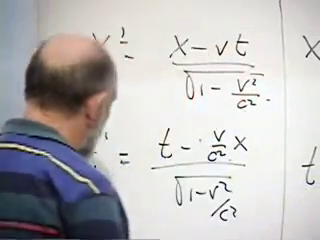
\includegraphics[width=0.76\textwidth]{lecture_01_figure_07.png}
\caption{\(c\) の因子を回復した後のローレンツ変換。}
\lectureframe{01:35:58}
\end{figure}

ただちに二つの確認ができる。まず \(v\ll c\) ととる。すると \(v^2/c^2\) は無視でき、通常の距離に対しては同時性の相対性の項 \(vx/c^2\) もまた無視できる。式~\eqref{eq:lorentz-dimensional}は
\begin{equation}
t'\approx t,\qquad x'\approx x-vt.
\end{equation}
に帰着する。ガリレイ相対性は低速近似として回復される。

第二に、光線を試す。\(c\) を回復すれば、右向きの光線は \(x=ct\) に従い、\(x=t\) ではない。代入すると
\begin{align}
x'&=\frac{(c-v)t}{\sqrt{1-v^2/c^2}},\\
t'&=\frac{(1-v/c)t}{\sqrt{1-v^2/c^2}}.
\end{align}
\(c-v=c(1-v/c)\) であるから、
\begin{equation}
x'=ct'.
\end{equation}
ダッシュ付きの観測者は同じ速さ \(c\) を測る。左向きの光線については、\(x=-ct\) を代入すれば同様に
\begin{equation}
x'=-ct'.
\end{equation}
が得られる。この変換はどちらの向きに進む光も正しく扱う。

\(x=t\) と \(x=ct\) の区別は、示唆に富む次元の確認である。前者は \(c=1\) となる単位系でのみ正しい。変換において通常の単位を回復しながら光線の方程式を自然単位のままにしておくと、二つの規約が混ざり、誤った結果を生む。次元の整合性はその誤りをただちに捉える。

\section{中点の判定基準}

\begin{classroomqa}
\audiencequestion{ある観測者が二つの閃光を同じ瞬間に受け取ったが、それらの光源の中間点にはいないとする。その観測者は、閃光が同時に発せられたと結論してよいだろうか。
\lecturetimestamp{01:42:55}}
\lecturerresponse{否。到着時刻が等しいことが発光時刻が等しいことを意味するのは、関連する座標系において二つの光源の空間的な中点にいる観測者だけである。一方の光源に近い受信者は、遠い方の閃光がより早く発せられていても、両方の閃光を一緒に受け取ることができる。運動する構成では、したがって中点の世界線 \(x=vt+L\) が本質的である。前方への光線 \(x=t\) をそれがその中点に出会うまで追い、次に後方への光線を \(x=vt+2L\) までたどる。その第二の端点の事象が、他の任意の等到着事象ではなく、運動する座標系によれば原点と同時である。}
\end{classroomqa}

われわれは完全な座標変換に到達したが、まだその最もよく知られた帰結には至っていない。次に続くのは長さの収縮、時間の遅れ、固有時間であり、さらに相対論的運動量とエネルギーが続く。基礎はすでに据えられている。各慣性系が同じ法則を用い、同じ光速を測ることができるのは、空間と時間が混ざり合い、遠方の同時性が世界に絶対的に属するのではなく座標系に属するからにほかならない。